\documentclass[a4paper]{article}
\usepackage{graphicx}
\usepackage{hyperref}

\begin{document}

\title{Analyzing Unoccupied Setback Effectiveness and Prevalence via K-Means Clustering}
\author{
	Jay Herron
	\and
	\url{https://github.com/NeedleInAJayStack/RTEM-Hackathon\_2022}
}
\date{\today}
\maketitle

\section{Intro}

Reducing energy use in buildings is expensive. Despite advances in fault-detection and diagnostic programs, achieving energy savings still requires manually evaluating issues to determine importance and making physical or virtual changes to rectify them. Because of this, better prioritization systems are needed.

Historically, energy reduction analytics can be separated into two categories:
\begin{enumerate}
\item{\textbf{Top-down}: Industry standard metrics like energy use intensity are used to compare buildings to their peers and grade their efficiency. While these are very useful for determining large energy users, they do little to suggest actions for energy reduction within a given building.}
\item{\textbf{Bottom-up}: Equipment-level analytics identify discrete operational issues, and include specific actions to take to resolve the issue. However, due to data availability issues and complex system interactions, energy savings estimates, when even provided, are unreliable.}
\end{enumerate}

There is an opportunity for a middle-of-the-road approach that uses high level metrics to analyze common low-level operational issues, and provides prioritization along with clear implementation guidelines.

This document proposes a set of key performance indicators (KPIs) and an analysis framework to identify and prioritize energy reduction through unoccupied setbacks. Nearly every building can achieve significant energy reductions by basic changes to their unoccupied operation, typically by modifying zone air temperature setpoints, minimum discharge air flow setpoints, or lighting based on occupancy. It is possible to implement these changes on nearly all controls equipment and the results are extremely cost-effective.

\section{Approach}

This framework requires whole-building energy use at hourly frequencies or faster. Whole-building energy usage is then cleaned by removing meter rollover artifacts, aligning time-stamps to a consistent frequency, and interpolating missing values. Next, the values are dis-aggregated if usage is represented by a monotonically increasing counter, and finally the history is passed through an outlier filter. After this process, we are left with clean, consistent energy usage data for the whole building.

Next, the cleaned data is split into weekly periods and each is passed through a k-means clustering algorithm\footnote{\url{https://en.wikipedia.org/wiki/K-means\_clustering}} that identifies 2 nodes: a high-usage cluster and a low-usage cluster. This process provides a mapping between each historical observation and whether it belongs in the high or low cluster, as well as average values for the high and low clusters. We interpret the high-usage period to be the occupied time in a building, and the low-usage period to be the unoccupied time.

From these results, we can compute two meaningful weekly KPIs:
\begin{enumerate}
\item{\textbf{Unoccupied Turndown Factor}: The high-usage cluster value divided by the low-usage cluster value. Scaled from 0 to 1, lower values indicate more effective unoccupied setbacks. Lower is better from an energy reduction standpoint.}
\item{\textbf{Occupied Duration Factor}: The amount of time the building was in a high-usage state, divided by the total time in the KPI period. Scaled from 0 to 1, lower values indicate more prevalent unoccupied setbacks, in terms of time.  Lower is better from an energy reduction standpoint.}
\end{enumerate}

This simple approach offers several distinct advantages. First, the data requirements are extremely low; only a single historical datastream for total energy use is required. Of the 230 buildings in the RTEM dataset, 99 have \textit{Electric Consumption} points, making it the 5th most prevalent point type behind \textit{Virtual}, \textit{Zone Temperature}, \textit{Outside Air Temperature}, and \textit{Status}. Second, it is widely applicable. The analysis process is not impacted by the type of building, the pattern of occupancy throughout the week, or the type of equipment within the building. Since no assumptions are made on the time of occupancy, it functions as well on irregularly occupied buildings (like community centers or theaters) as on regularly occupied buildings (like commercial office buildings or retail). Finally, it delivers actionable results. Even the most primitive control systems offer features for modifying building operation according to occupancy.

\section{Usage}

These KPIs alone do not scale according to energy usage, so they are best used as part of a top-down Energy Use Intensity-based analysis. For example, if comparing buildings within a portfolio, the EUI could be used to determine the worst-performing facilities, and then the KPIs above could be used to determine whether these facilities would benefit from improving the unoccupied operation.

The different KPIs suggest different actions:
\begin{itemize}
\item{A large Unoccupied Turndown Factor suggests that unoccupied operation should be investigated. When unoccupied, zone air temperature setpoint deadbands should widen significantly, minimum discharge airflow setpoints should be set to 0, and lights should be turned off. This KPI may also suggest that there are areas of the building that never enter an unoccupied state.}
\item{A large Occupied Duration Factor suggests that occupancy scheduling and detection systems should be investigated. Of course, unoccupied energy saving measures must conform to each building's unique occupancy patterns. However, if occupancy is based on a schedule, that schedule should be checked to ensure that it matches actual occupancy patterns. If occupancy is detected using a sensor, the sensors should be validated for correct operation.}
\end{itemize}

While a KPI value on a particular building during a particular week is meaningful, KPIs are typically most useful when they are compared between entities or over time. A building with a large KPI value compared to its peers, or with a KPI value that increases over time may provide context on what constitutes a "large" KPI value.

\section{Results}

% TODO: Remove point count
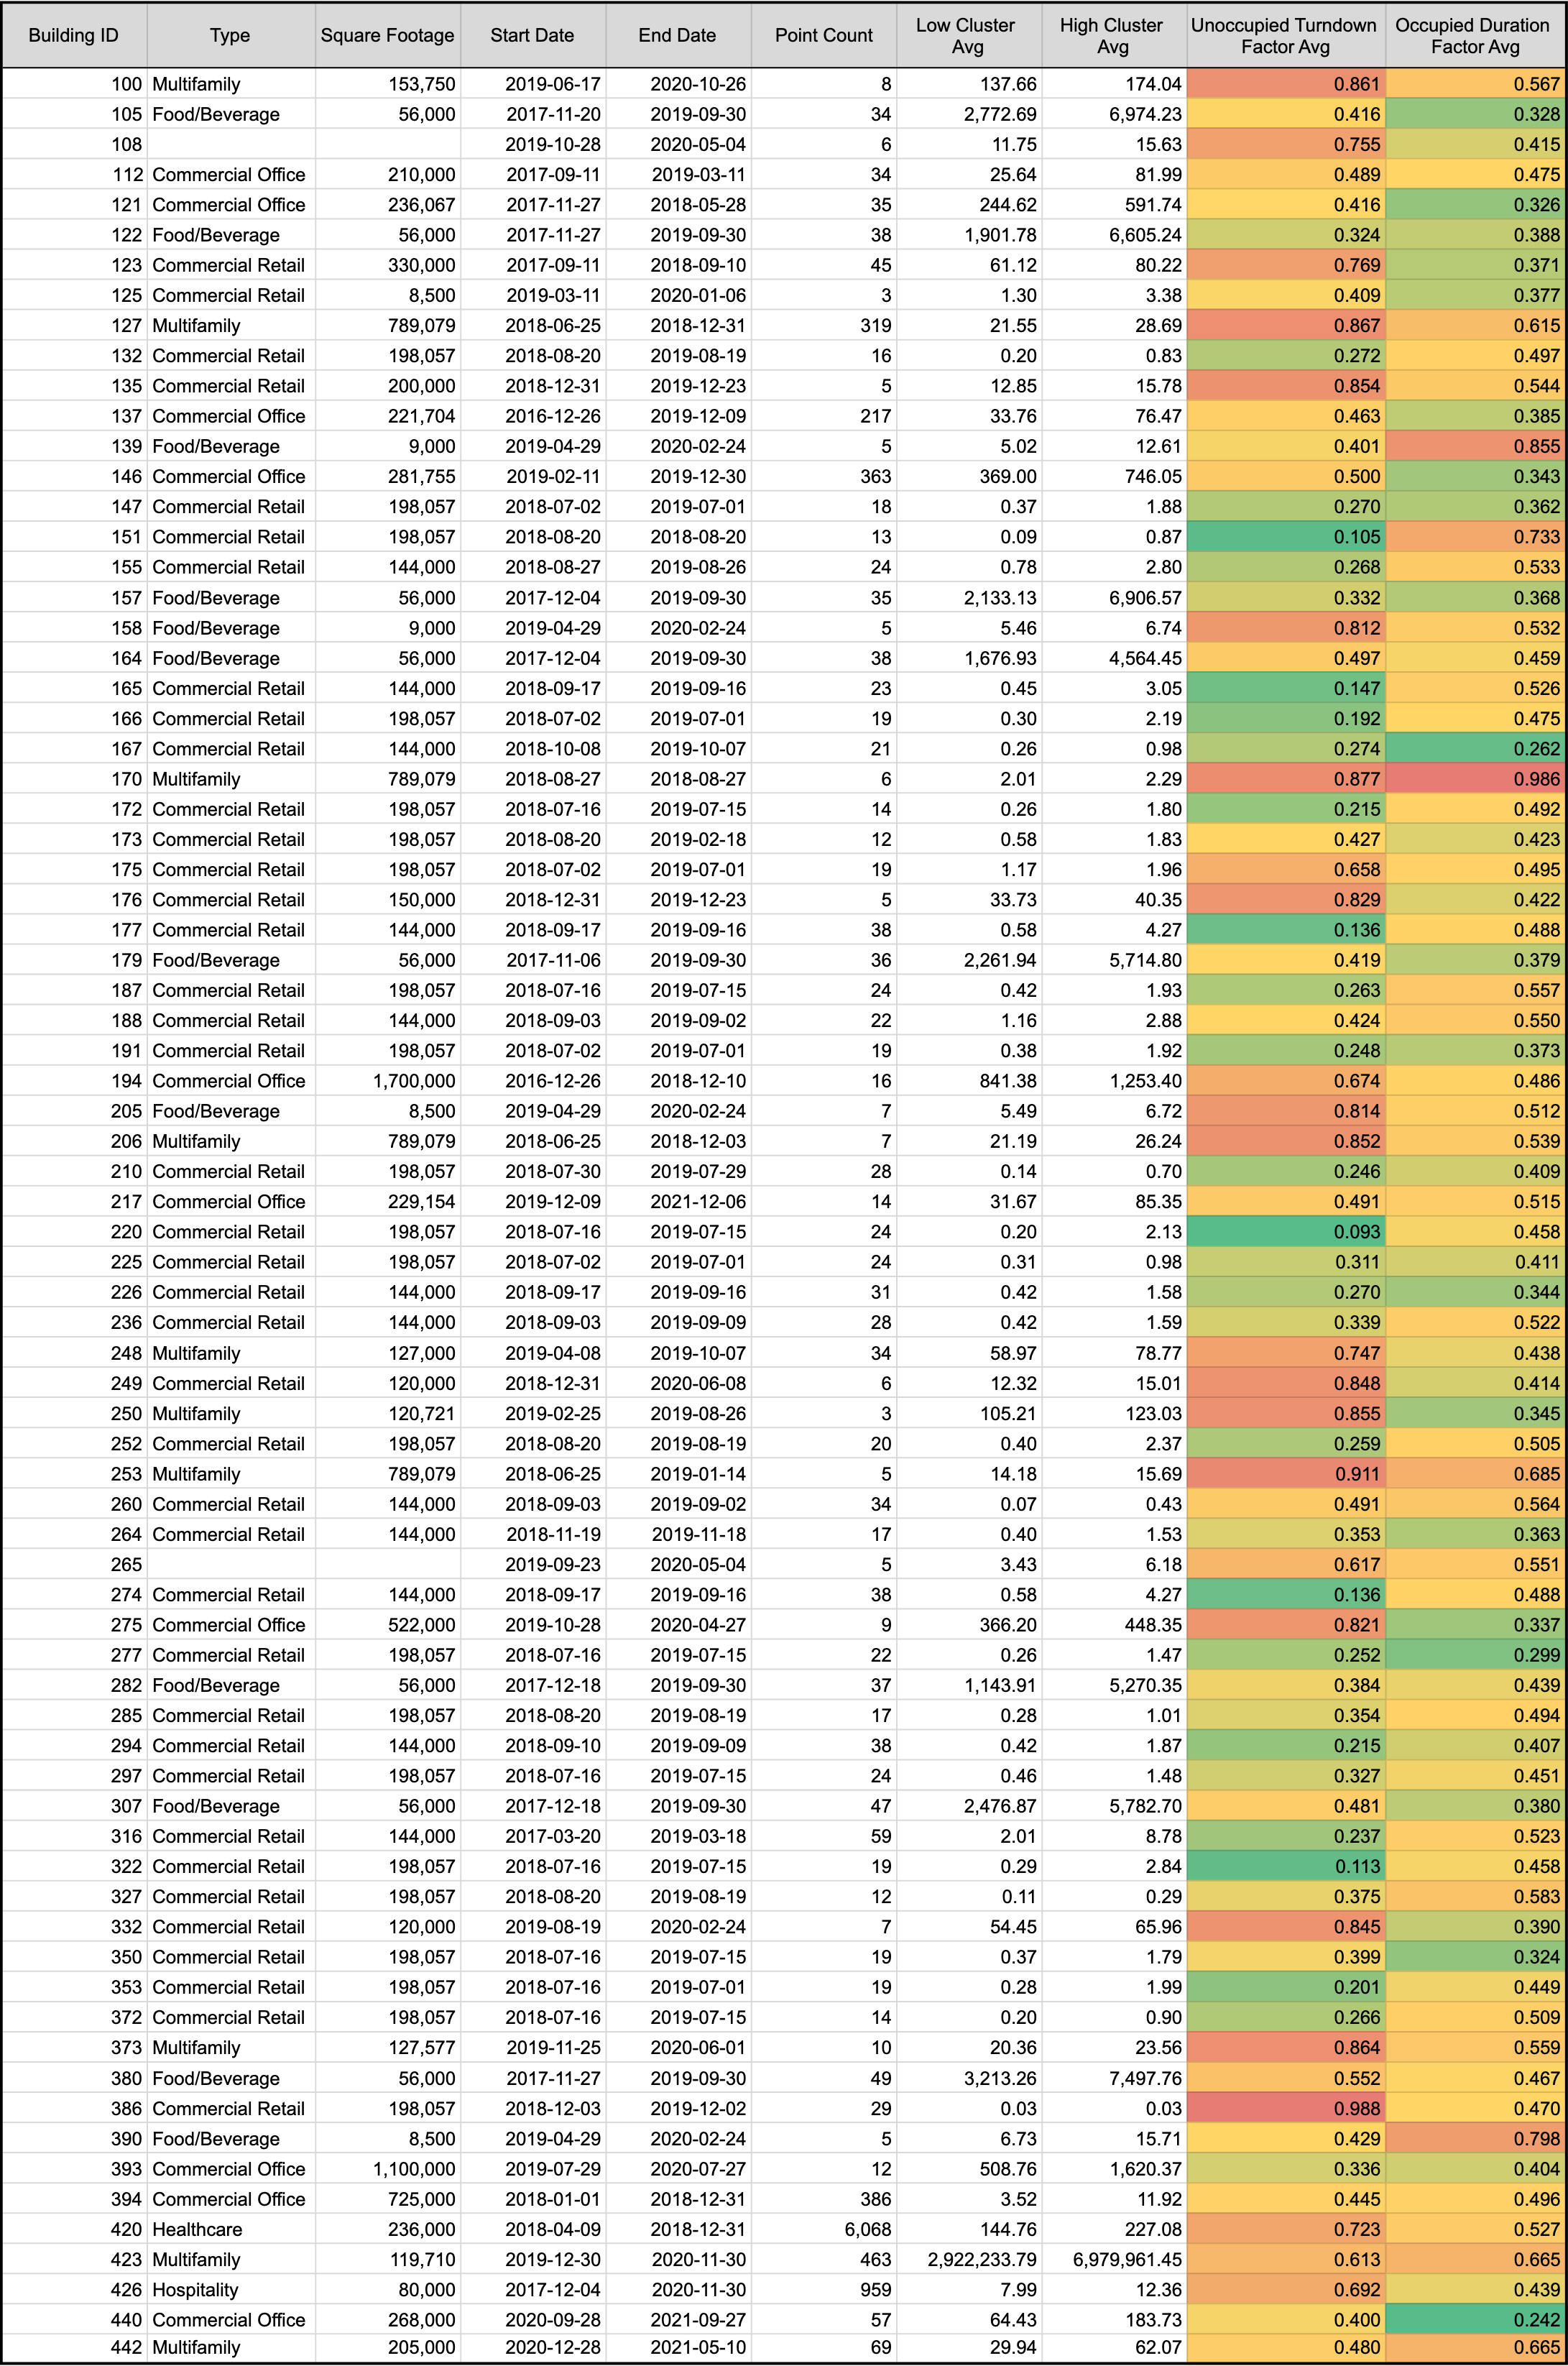
\includegraphics[width=\columnwidth]{./images/KPI_Result_Table.png}

\section{Analysis}

\subsection{Building 188}

Building 188 and Building 165 are similarly sized commercial retail spaces with similar occupied electricity consumption. However, Building 188 has an average Unoccupied Turndown Factor of 0.424 while Building 165 has a value of 0.147. By observing the respective usage over a representative week in June 2019, we can indeed see larger energy consumption in Building 188 during unoccupied times.

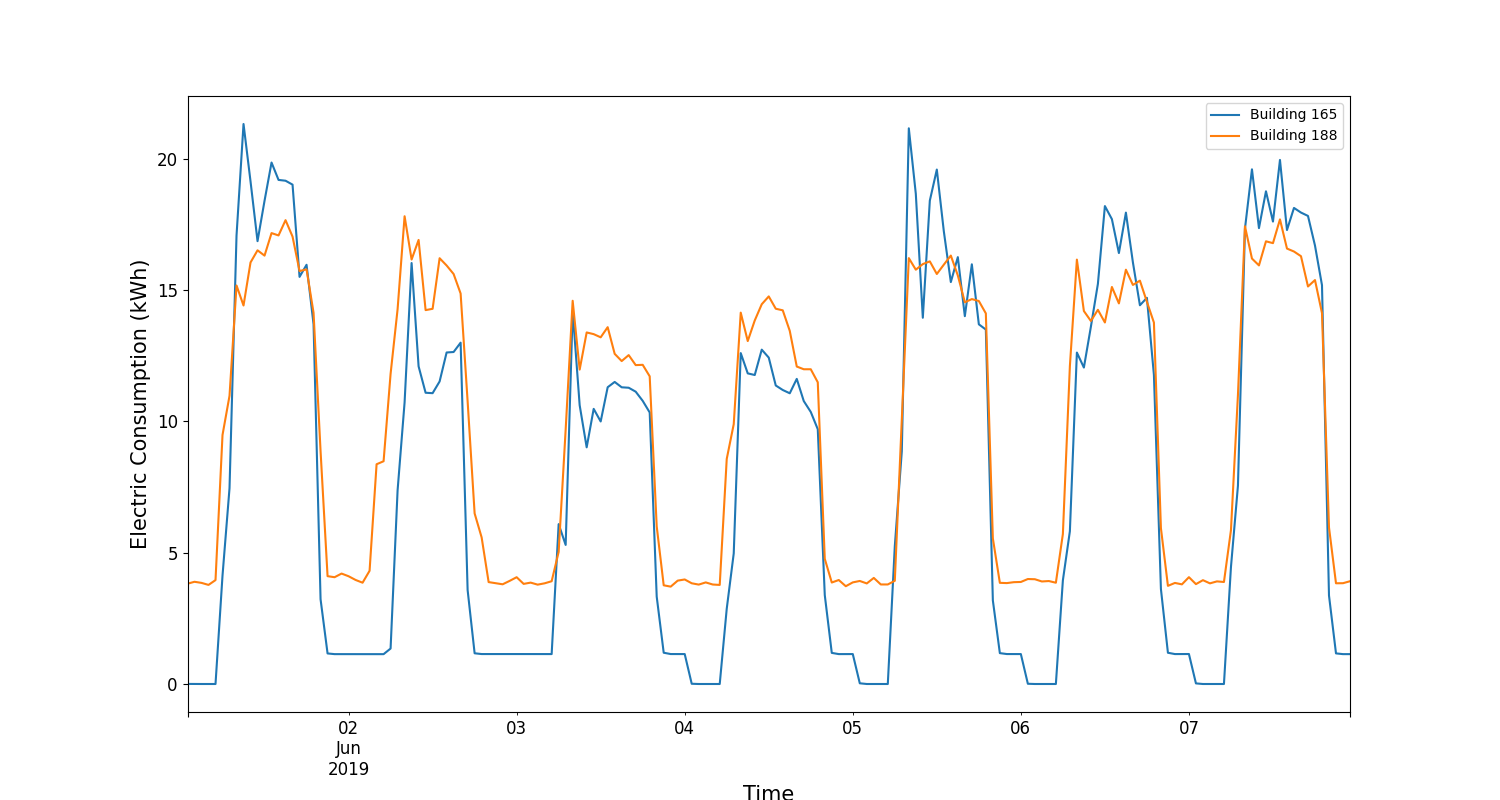
\includegraphics[width=.8\columnwidth]{./images/188v165_Turndown.png}

Since these facilities have HVAC submetering, we can start to disaggregate the total electricity consumption. By charting the total HVAC energy use over the same timeframe, we find that the nighttime usage in Building 188 is unrelated to the HVAC equipment, suggesting that it is likely related to light or plug loads

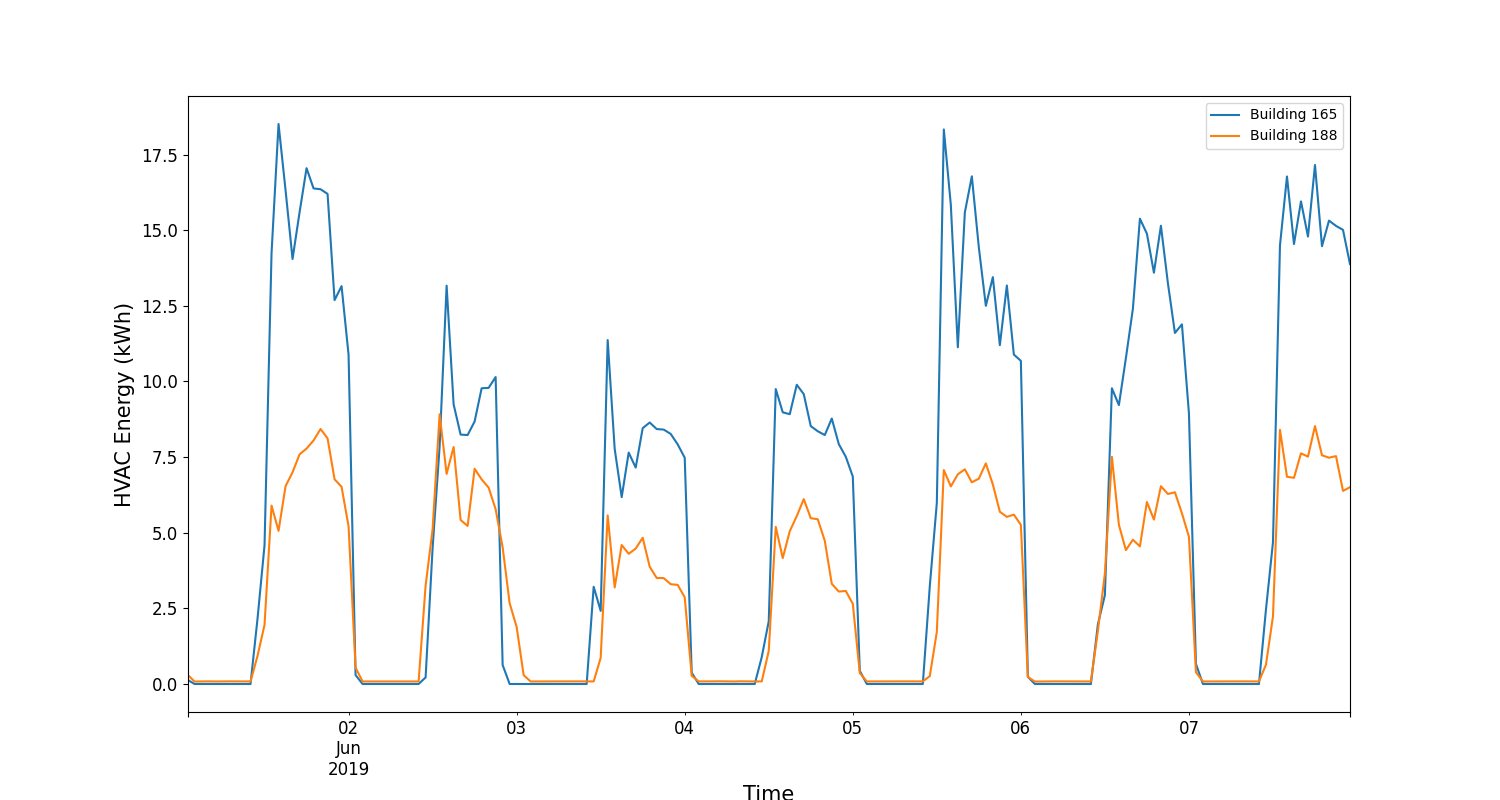
\includegraphics[width=.8\columnwidth]{./images/188v165_Turndown_HVAC.png}

If Building 188 is able to achieve a turndown equivalent to that of Building 165, the KPIs suggest that its energy consumption will be reduced by about 11,500 kilowatt-hours (kWh) per year, which is roughly 16\% of its total yearly energy usage.

\subsection{Building 275}

Building 275 and 393 are both large office buildings. Building 393 has more than twice the square footage and three times the occupied electrical consumption of 275. However, with an unoccuiped turndown factor of 0.821, Building 275 has much less effective unoccupied setbacks than Building 393, whose factor is 0.336. By charting their usage together for a week in early March 2020, we can see the difference in the unoccupied consumption.

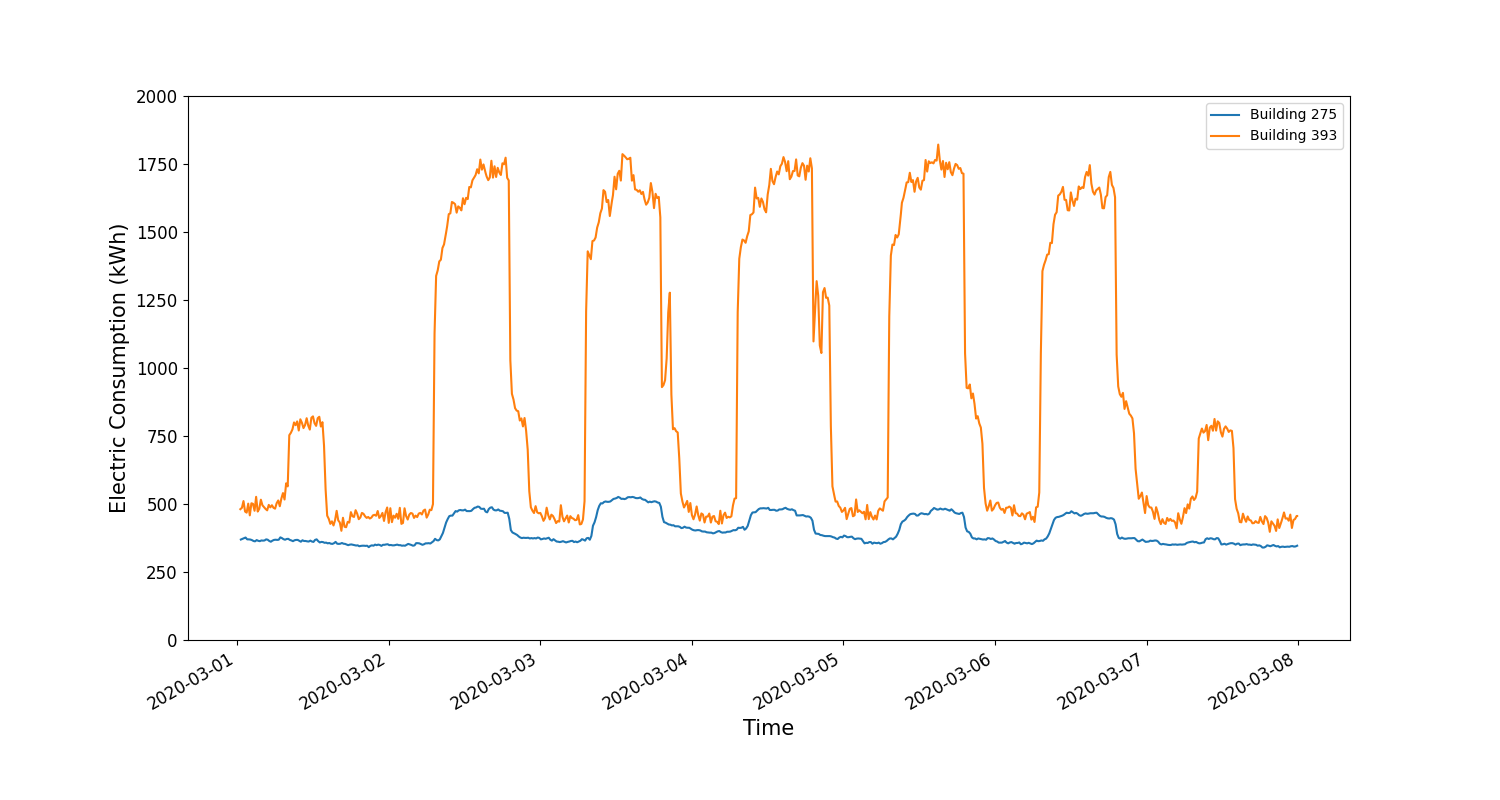
\includegraphics[width=.8\columnwidth]{./images/275v393_Turndown.png}

If Building 275 was able to achieve the same unoccupied turndown factor as 393, which is not unusual in the commercial office group, it would reduce its total energy use by an estimated 36\%. Extrapolating from the 6 months of available energy usage data, this would result in savings of 5,000,000 kWh or nearly \$750,000 of reduced consumption charges per year, based on a 15-cent per kWh cost.

\subsection{Building 390}

Building 390 is a food and beverage facility, with a large occupied duration factor of 0.798. An investigation of the eletrical consumption over a week in July 2019 shows that usage is high from roughly 4AM to midnight each evening.

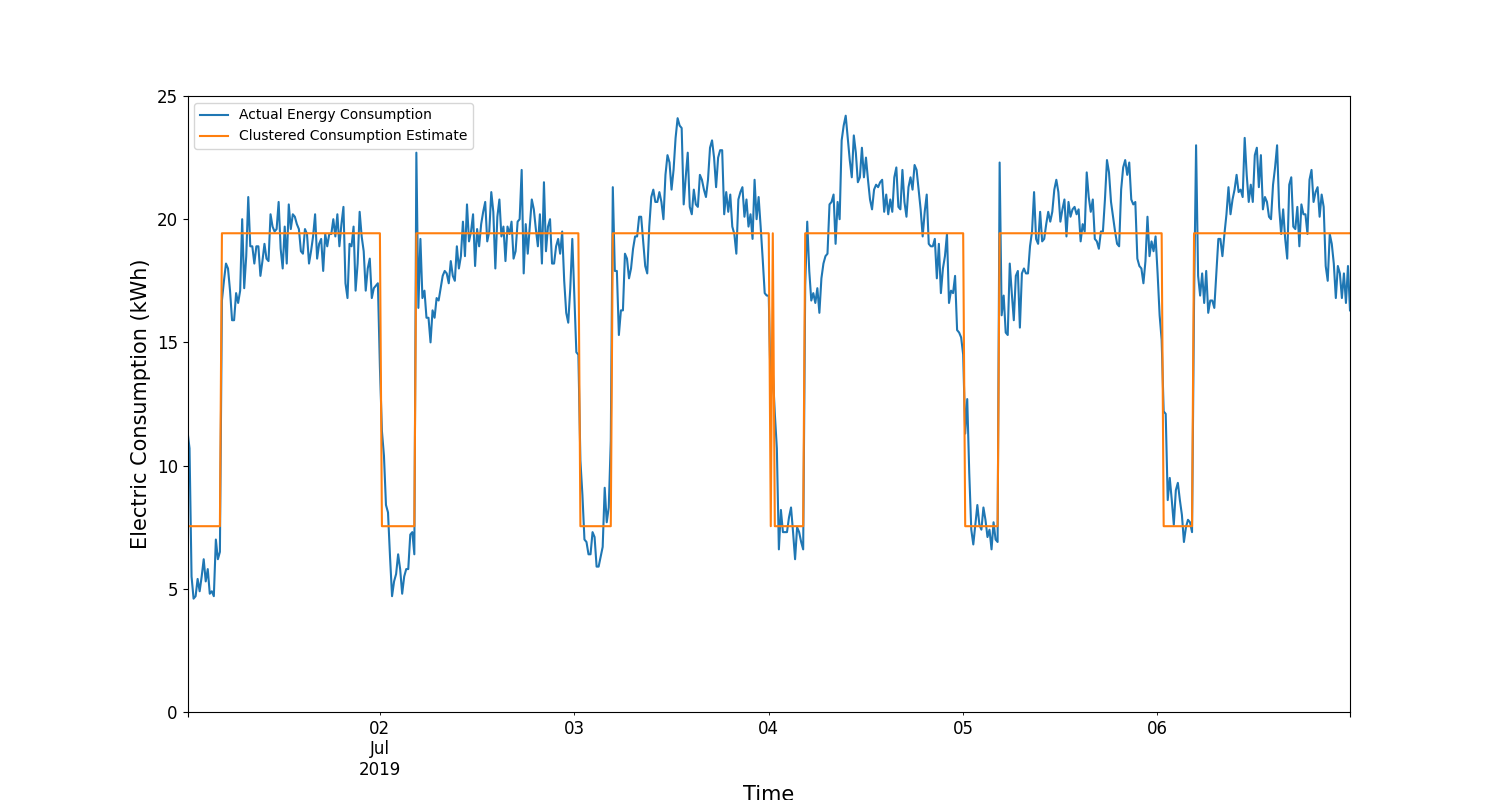
\includegraphics[width=.8\columnwidth]{./images/390_Duration.png}

There are certainly food and beverage facilities that keep these hours, as staff prep in the morning and clean up at night. However a quick investigation could determine if the consumption profile reflects actual occupancy schedules. If not, and the building could be run in an unoccupied mode even just 2 additional hours each day, that would save nearly 5\% of this building's total energy consumption.

\section{Future Growth}

% TODO: Provide more specific guidance on how to use on future expansion

As the RTEM dataset expands, these weekly KPIs can be automatically computed on new data. In fact, computing KPI values for the complete RTEM dataset throughout all time currently takes only a few minutes on commodity hardware. Scripts to compute these KPIs are provided in the GitHub repository linked below the title.

However, the automation of this process suffers from incomplete data modeling of electrical metering within the RTEM dataset. For example, given a site with multiple electric consumption readings, it is not denoted whether a specific reading is a subset of another or fully separate. Top level consumption readings are not differentiated from low-level submeters. Due to this, the final point list used within the analysis was manually revised to determine which points (or collection of points) represented each building as a whole. Project Haystack models metering trees using the \texttt{submeterOf}\footnote{\url{https://project-haystack.org/doc/lib-phIoT/submeterOf}} tag, and denotes top-level metering using a \texttt{meterScope}\footnote{\url{https://project-haystack.org/doc/lib-phIoT/meterScope}} tag. Brick Schema models building-level meters with a \texttt{Building\_Meter}\footnote{\url{https://brickschema.org/ontology/1.2/classes/Building\_Meter}} class. Integration of these ideas into the RTEM dataset would improve future automation efforts.

\section{Additional Applications}

% TODO: Expand a bit on each application

The clustering approach shown in this document is not specific to total-building electric energy use. It could potentially be applied in very similar ways to:
\begin{itemize}
\item{Other building-level utilities: Total building gas, chilled water, or steam use}
\item{Submetering: Zone or tenant-level unoccupied setback analysis and tracking}
\item{Downstream occupancy effectiveness metrics: Zone air temperature setpoints, VAV discharge airflow}
\end{itemize}

\section{Conclusion}

This document presents a strategy for analyzing the effectiveness and prevalence of unoccupied setbacks by using a clustering algorithm on a historical whole-building consumption record. It outlines the KPIs that can be calculated from this record, and demonstrates how they can be used on real-world data from the RTEM dataset. Finally, it discusses the feasibility of expanding this analysis as the RTEM dataset grows.

% TODO: Align the conclusion with the introduction

Energy conservation is the most cost-effective means of decarbonization. Of course, investments must be made in switching fossil fuel-based technologies to clean energy, and expanding renewable energy production. However, in the meantime, we must also make sure that our existing infrastructure is working as efficiently and effectively as possible. Poor unoccupied operation is the largest opportunity in most buildings that does not require a capital investment. We ought to make sure it is working well and continues to do so.

\end{document}